\begin{figure*}

\begin{subfigure}{0.425\linewidth}
\centering

\includegraphics[width=\linewidth,trim=0 0.2cm 0 0,clip]{../binder/binder-bucket=prq49--a=all_stints_all_series_profiles+endeavor=16--fitness_complexity.ipynb/binder/teeplots/bucket=prq49--a=all_stints_all_series_profiles+endeavor=16--fitness_complexity/annot=morph+hue=series+viz=lineplot+what=16005+x=stint+y=flagged-advantageous-sites+ext=.pdf}

\vspace{-1ex}

\caption{\footnotesize genotype complexity, case study (blue) vs. others}
\label{fig:16005-timelapse:genotype-complexity}
\end{subfigure}%
\begin{subfigure}{0.425\linewidth}
\centering

\includegraphics[width=\linewidth,trim=0 0.2cm 0 0,clip]{../binder/binder-bucket=prq49--a=all_stints_all_series_profiles+endeavor=16--interface_complexity.ipynb/binder/teeplots/bucket=prq49--a=all_stints_all_series_profiles+endeavor=16--interface_complexity/annot=morph+hue=series+viz=lineplot+what=16005+x=stint+y=cardinal-interface-complexity+ext=.pdf}

\vspace{-1ex}

\caption{\footnotesize phenotype complexity, case study (blue) vs. others}
\label{fig:16005-timelapse:phenotype-complexity}
\end{subfigure}%
\begin{subfigure}{0.15\linewidth}
\centering

\includegraphics[width=\linewidth,trim=1cm 0.15cm 0.8cm 0,clip]{../binder/binder-bucket=prq49--a=all_stints_all_series_profiles+endeavor=16--fitness_complexity.ipynb/binder/teeplots/bucket=prq49--a=all_stints_all_series_profiles+endeavor=16--fitness_complexity/how=mean+hue=series+inner=box+iqr=shade+viz=scatterplot+what=16005+x=flagged-advantageous-sites+y=cardinal-interface-complexity+ext=.pdf}

\vspace{-1ex}

\caption{\footnotesize mean g.c./p.c.}
\label{fig:16005-timelapse:mean-complexity}
\end{subfigure}

\begin{tcolorbox}[
  enhanced,
  colframe=morphj!30!white,
  colback=morphj!4!white,
  boxrule=0.8pt,
  arc=1pt,
  boxsep=0pt,
  left=0pt,right=0pt,top=0pt,bottom=0pt,
  width=\linewidth,
]
\savebox{\morphjtitlebox}{%
  \begin{tabular}{@{}c@{}}
    \bfseries\footnotesize morph~\tikz[baseline=(morphjbadge.base)]{%
      \node[draw=black,very thick,fill=morphj,circle,inner sep=1pt,minimum size=1.1em,text=white] (morphjbadge) {$\boldsymbol{j}$};%
    }\\[2pt]
    \bfseries\footnotesize life history\\[3pt]
    \scriptsize video animation:\\[-2pt]
    \scriptsize\href{https://hopth.us/hr}{\texttt{\scriptsize hopth.us/hr}}
  \end{tabular}%
}
% each of the 5 panels is 0.2\panelcolwd wide and holds a picture set at
% 0.9 of that, so 0.01\panelcolwd of slack already sits at the column's
% outer edge; leading the panel row with the same amount gives the frame
% the same clearance on top and right
\setlength{\panelcolwd}{\dimexpr\linewidth-\wd\morphjtitlebox-12pt\relax}
\setlength{\panelpad}{0.01\panelcolwd}
% The pictures are cropped, so how tall they come out is not something to
% assume; set one and measure it.
\savebox{\panelimgbox}{%
  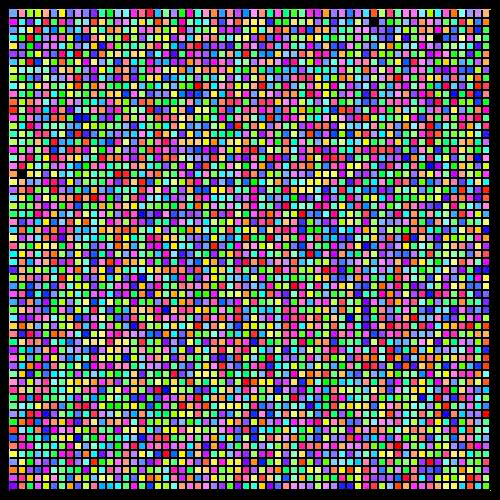
\includegraphics[width=0.18\panelcolwd,trim=4cm 4cm 4cm 4cm,clip]{img/a=kin-group-id+idx=0+proc=0+series=16005+stint=100+thread=0+update=16-8752_16/frame_0001.png}%
}
\setlength{\panelimght}{\dimexpr\ht\panelimgbox+\dp\panelimgbox\relax}
% a specimen subcaption, twice: strutted, to measure the line it is set
% on, and bare, to measure how far its letters actually reach.
% The difference is the slack the line leaves over and under them, which
% counts towards the white space the reader sees.
\savebox{\panelcapbox}{\footnotesize\strut(h) update 952}
\savebox{\panelcapinkbox}{\footnotesize(h) update 952}
% A probe panel: the same picture captioned the same way, but unnumbered,
% so it steps no counter and writes no list-of-figures entry.
% What it holds beyond the picture and that line is the skip the caption
% package leaves above a subcaption, which differs between TeX
% distributions --- so the figure tightens it by proportion below rather
% than replacing it with a length of its own.
\savebox{\panelprobebox}{%
  \begin{subfigure}{0.2\panelcolwd}
  \centering
  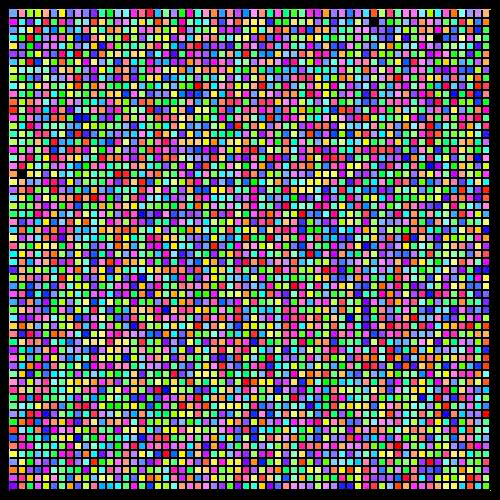
\includegraphics[width=0.9\linewidth,trim=4cm 4cm 4cm 4cm,clip]{img/a=kin-group-id+idx=0+proc=0+series=16005+stint=100+thread=0+update=16-8752_16/frame_0001.png}%
  \caption*{update 8}
  \end{subfigure}%
}
\setlength{\panelcapskip}{\dimexpr\ht\panelprobebox+\dp\panelprobebox
  -\panelimght-\ht\panelcapbox-\dp\panelcapbox\relax}
% the white space actually on show above and below a subcaption
\setlength{\panelcapabove}{\dimexpr\panelcapskip
  +\ht\panelcapbox-\ht\panelcapinkbox\relax}
\setlength{\panelcapbelow}{\dimexpr\panelcapskip
  +\dp\panelcapbox-\dp\panelcapinkbox\relax}
% take a third off the gap above the subcaptions and half off the gap
% below them, both measured as seen
\setlength{\panelcaptrim}{0.33\panelcapabove}
\setlength{\panelcappad}{0.5\panelcapbelow}
\addtolength{\panelcappad}{\dimexpr\dp\panelcapinkbox-\dp\panelcapbox\relax}
% Save the panel row so its height is measured rather than derived from
% lengths that vary between TeX distributions.
\savebox{\panelrowbox}{%
\begin{subfigure}{0.2\panelcolwd}
\centering
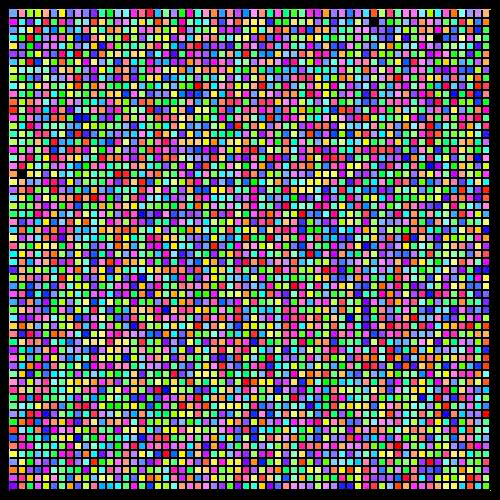
\includegraphics[width=0.9\linewidth,trim=4cm 4cm 4cm 4cm,clip]{img/a=kin-group-id+idx=0+proc=0+series=16005+stint=100+thread=0+update=16-8752_16/frame_0001.png}%
\vspace{-\panelcaptrim}%
\caption{update 8}
\label{fig:16005-timelapse:update64}
\end{subfigure}%
\begin{subfigure}{0.2\panelcolwd}
\centering
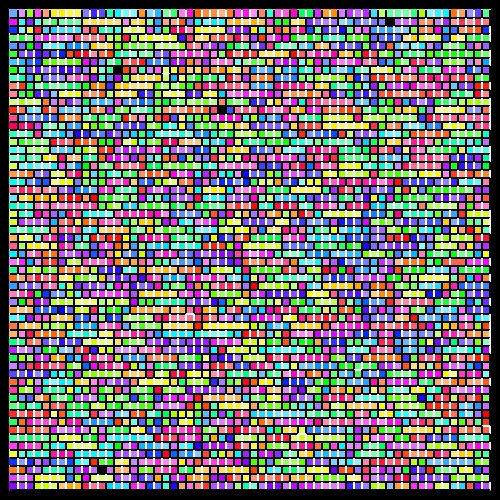
\includegraphics[width=0.9\linewidth,trim=4cm 4cm 4cm 4cm,clip]{img/a=kin-group-id+idx=0+proc=0+series=16005+stint=100+thread=0+update=16-8752_16/frame_0016.png}%
\footnotesize
\vspace{-\panelcaptrim}%
\caption{update 32}
\label{fig:16005-timelapse:update256}
\end{subfigure}%
\begin{subfigure}{0.2\panelcolwd}
\centering
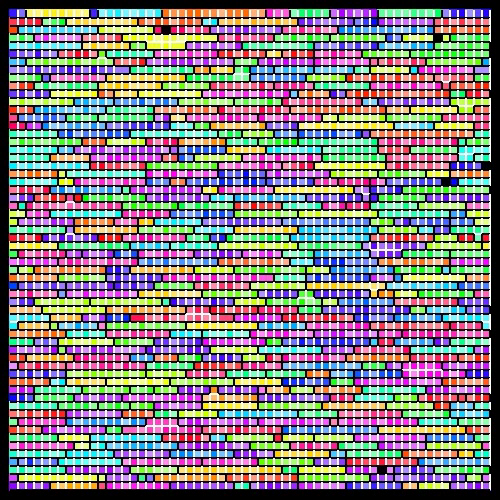
\includegraphics[width=0.9\linewidth,trim=4cm 4cm 4cm 4cm,clip]{img/a=kin-group-id+idx=0+proc=0+series=16005+stint=100+thread=0+update=16-8752_16/frame_0052.png}%
\footnotesize
\vspace{-\panelcaptrim}%
\caption{update 104}
\label{fig:16005-timelapse:update832}
\end{subfigure}%
\begin{subfigure}{0.2\panelcolwd}
\centering
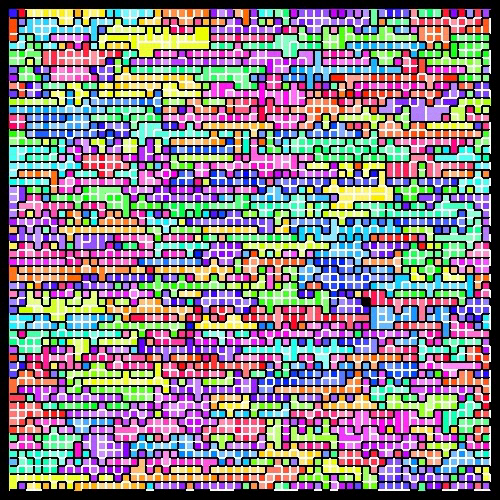
\includegraphics[width=0.9\linewidth,trim=4cm 4cm 4cm 4cm,clip]{img/a=kin-group-id+idx=0+proc=0+series=16005+stint=100+thread=0+update=16-8752_16/frame_0420.png}%
\footnotesize
\vspace{-\panelcaptrim}%
\caption{update 840}
\label{fig:16005-timelapse:update6720}
\end{subfigure}%
\begin{subfigure}{0.2\panelcolwd}
\centering
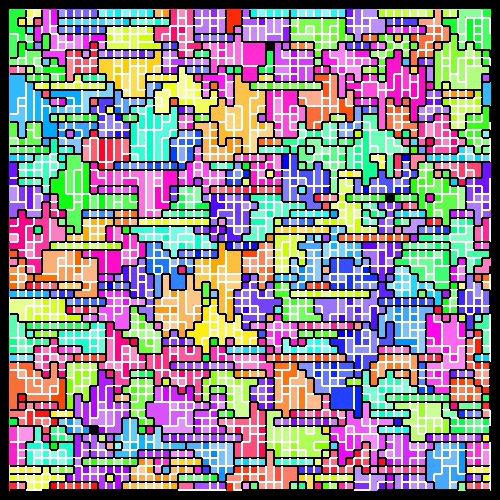
\includegraphics[width=0.9\linewidth,trim=4cm 4cm 4cm 4cm,clip]{img/a=kin-group-id+idx=0+proc=0+series=16005+stint=100+thread=0+update=16-8752_16/frame_0476.png}%
\footnotesize
\vspace{-\panelcaptrim}%
\caption{update 952}
\label{fig:16005-timelapse:update7616}
\end{subfigure}%
}
\setlength{\panelrowht}{\dimexpr\panelpad+\ht\panelrowbox+\dp\panelrowbox
  +\panelcappad\relax}
\setlength{\tabcolsep}{0pt}
\renewcommand{\arraystretch}{1}
\begin{tabular}{@{}>{\cellcolor{morphj!25!white}}m{\dimexpr\wd\morphjtitlebox+8pt\relax}@{\hspace{4pt}}m{\panelcolwd}@{}}
% Both cells are boxes of the same measured height, so they line up top
% and bottom whatever the surrounding lengths happen to be; the title
% then centers on the pictures by sitting in a box exactly as tall as
% they are.
\parbox[c][\panelrowht][t]{\dimexpr\wd\morphjtitlebox+8pt\relax}{%
  \vspace*{\panelpad}%
  \vbox to \panelimght{%
    \vfil
    \hbox to \linewidth{\hfil\usebox{\morphjtitlebox}\hfil}%
    \vfil
  }%
}
&
\parbox[c][\panelrowht][t]{\panelcolwd}{%
  \vspace*{\panelpad}%
  \usebox{\panelrowbox}%
}
\\
\end{tabular}

\end{tcolorbox}

\vspace{-1.5ex}

\caption{%
\textbf{Case study strain.}
\footnotesize
Compared to other replicates, case study 16005 sustained extreme outlying complexity (upper panels \labelcref{fig:16005-timelapse:genotype-complexity,fig:16005-timelapse:phenotype-complexity,fig:16005-timelapse:mean-complexity}) and exhibited unique multi-stage patterned growth (lower panels \labelcref{fig:16005-timelapse:update64,fig:16005-timelapse:update256,fig:16005-timelapse:update832,fig:16005-timelapse:update6720,fig:16005-timelapse:update7616}).
Genotype complexity counts genome sites contributing to fitness; phenotype complexity counts distinct cell input/output operations contributing to fitness --- both determined via knockout/interference trials.
Snapshots show example life history (morph ``$j$,'' transfer round 100; Supplementary Table \ref{tab:morph_descriptions}).
Hue denotes, and black borders divide, multicell groups; white borders reflect inner structure.
From initial unicell groups (\ref{fig:16005-timelapse:update64}), cells replicate to form horizontal ``cigar-like'' bodies (\labelcref{fig:16005-timelapse:update256,fig:16005-timelapse:update832}).
In a delayed second stage of growth, groups expand vertically to produce a ``box-like'' final morphology (\labelcref{fig:16005-timelapse:update6720,fig:16005-timelapse:update7616}).
During this secondary phase of growth, some groups establish cigar-like propagules (\labelcref{fig:16005-timelapse:update7616}).
}
\label{fig:16005-timelapse}

\end{figure*}
